% !TEX root = main.tex

\section{Implementierung}
%TODO Text ergänzen
\subsection{Sequentiell}
Die erste und einfachste Umsetzung des Entwurfs des Simulationsschritts wäre folgendes:
\begin{lstlisting}[language=C]
for (int i = 1; i < arrLen-1; i++)
	newval[i] = (2 * values[i]) - oldval[i] + c * (values[i-1] - (2 * values[i]) + values[i+1]);

for (int i = 1; i < arrLen-1; i++) 
{
	oldval[i] = values[i];
	values[i] = newval[i];
}
\end{lstlisting}

Dabei führen wir die Berechnung durch und kopieren anschließend die Werte jeweils einen "Schritt in die Vergangenheit". Das Kopieren der Arrays stellt unnötige Schreiboperationen dar. Eine Alternative hierzu ist der Toggle:

\begin{lstlisting}[language=C]
for (int i = 1; i < arrLen-1; i++)
{
	if (0 == mode)
		newval[i] = (2 * values[i]) - oldval[i] + c * (values[i-1] - (2 * values[i]) + values[i+1]);
	else if (1 == mode)
		oldval[i] = (2 * newval[i]) - values[i] + c * (newval[i-1] - (2 * newval[i]) + newval[i+1]);
	else
		values[i] = (2 * oldval[i]) - newval[i] + c * (oldval[i-1] - (2 * oldval[i]) + oldval[i+1]);
}
mode++;
if (2 < mode)
	mode = 0;
\end{lstlisting}

Hierbei wird kein Array auf ein anderes kopiert. Stattdessen wird die Bedeutung der Arrays verschoben. Initial werden auf newval die berechneten Werte geschrieben, values hält die gegenwärtigen Werte und oldval die ältesten Werte. Nach jedem Simulationsschritt wird dann die Bedeutung verschoben. Somit werden dann im nächsten Schritt die neuen Werte in oldval geschrieben, newval hält die gegenwärtigen Werte und values die ältesten Werte.\\
In Abbildung \ref{fig:toggle_swap} ist das Prinzip der Semantikverschiebung beim Toggle dargestellt.\\

\begin{figure}[H]
	\centering
	\smartdiagram[circular diagram:clockwise]{newval, values, oldval}
	\caption{Verschiebung der Semantik der Arrays}
	\label{fig:toggle_swap}
\end{figure}

\subsection{OpenMP}
Die Parallelisierung mit OpenMP ist nun sehr einfach. Dem Quellcode muss nur eine Zeile hingefügt werden und die Schleife wird dann parallelisiert:

\begin{lstlisting}[language=C]
#pragma omp parallel for
for (int i = 1; i < arrLen-1; i++)
[...]
\end{lstlisting}

In diesem Fall werden alle Variablen bis auf "i", da diese erst im Scope der Schleife deklariert wird, als global oder shared angesehen. Wir hatten hier die Vermutung, dass wir deshalb auch vom False-Sharing-Problem betroffen sein könnten. Aufgrund der Größe der Arrays und der Art wie OpenMP die Arrays aufteilt sollte dies aber nicht der Fall sein.

\subsection{OpenMPI}
Die Implementierung der verteilten Wellensimulation hat einige Änderungen und Ergänzungen am Basiscode des Projekts nötig gemacht. So wird die Simulationsfunktion fortan für ein abgestecktes Interval von linken zum rechten Ende des vorgegebenen Bereich durchgeführt. Damit wird sichergestellt, dass jeder Worker-Thread ausschließlich den eigenen Simulationsbereich bearbeitet.

\begin{lstlisting}[language=C]
void simulate(int leftEnd, int rightEnd)
{
for (int i = leftEnd; i < rightEnd; i++)
{
	newval[i] = (2 * values[i]) - oldval[i] + c * (values[i - 1] - (2 * values[i]) + values[i + 1]);
}
\end{lstlisting}

Um den Nachrichtenaustausch zwischen Master- und Worker-Threads übersichtlicher zu gestalten wurden Wrapper-funktionen, die den gesamten Kommunikationsprozess verwalten, entwickelt. Jede dieser Wrapper-funktionen besitzt dabei einen Antagonisten. Hierbei gehören die Funktionen scatterChunksToWorker und rxChunkFromMaster, sowie collectChunksFromWorkers und txChunksToMaster untrennbar zusammen. Durch den Aufruf einer dieser Funktionen auf der Master- oder Worker-Seite wird ein Aufruf der Antagonisten für den fehlerfreien Ablauf der Simulation verpflichtend.

\begin{figure}[H]
	\centering
	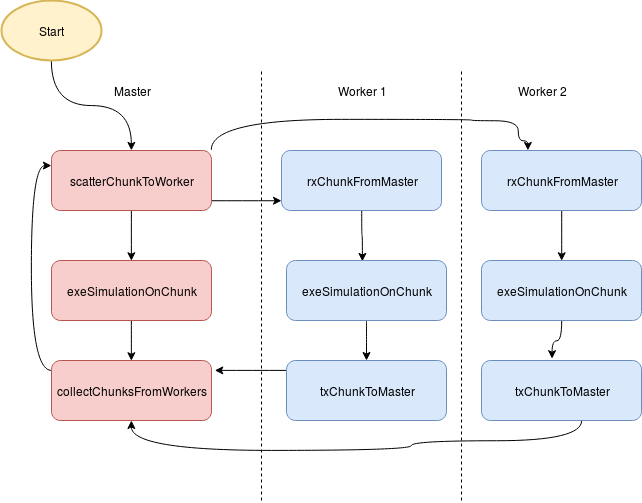
\includegraphics[width=1\textwidth]{pictures/MessagePassingManagement.png}
	\caption{Management der Kommunikations}
	\label{fig:ManagementMessages}
\end{figure}

Die Wrapperfunktionen verwenden hierbei bei der Ausführung die OpenMPI-Funktionen Send und Receive, welche im Kapitel 2.4 näher erläutert wurden. Exemplarisch wird der Nachrichtenaustausch am Beispiel der nachfolgenden Code-fragmente der Funktionen CollectChunkFromWorker und txChunkToMaster beleuchtet.

\begin{lstlisting}[language=C]
void txChunksToMaster()
{
	MPI_Send(&offset, 1, MPI_INT, MASTER, 0, MPI_COMM_WORLD);
	MPI_Send(&oldval[offset], chunksize, MPI_DOUBLE, MASTER, 0, MPI_COMM_WORLD);
	MPI_Send(&values[offset], chunksize, MPI_DOUBLE, MASTER, 0, 	MPI_COMM_WORLD);
}
\end{lstlisting}

Die Funktion txChunksToMaster birgt die Sendefunktionen und wird ausschließlich von Worker-Threads aufgerufen. Das Sendeziel bildet hierbei der Master-Thread. Bei der Ausführung der Funktion wird zuerst das Worker-eigenen Offset des simulierten Wellenabschnittes übertragen. Danach werden zwei Arrays der Länge des eines Chunks übermittelt. Die übertragenen Arrays sind die alten und aktuellen Werte des zugeteilten Wellenabschnittes. Sinnvoll wird der Aufruf von txChunkToMaster erst nach der Ausführung eines Simulationsschrittes mit Hilfe der Funktion exeSimulationOnChunk.   

\begin{lstlisting}[language=C]
void collectChunksFromWorkers(int numtasks)
{
	for (int source = 1; source < numtasks; source++)
	{
		MPI_Recv(&offset, 1, MPI_INT, source, 0, MPI_COMM_WORLD, &status);
		MPI_Recv(&oldval[offset], chunksize, MPI_DOUBLE, source, 0, MPI_COMM_WORLD, 	&status);
		MPI_Recv(&values[offset], chunksize, MPI_DOUBLE, source, 0, MPI_COMM_WORLD, 	&status);
	}
}
\end{lstlisting}

Der Antagonist zu txChunksToMaster stellt die Funktion collectChunksFromWorkers dar. Hierbei werden alle Chunks der Worker-Threads eingesammelt. Das Einsammeln wird mit der Funktion Receive realisiert. Zuerst wird das Offset des jeweilig sendenen Worker-threads empfangen. Dadurch kann für die nachfolgend empfangenen Arrays ein Update der richtigen Punkte des Master-thread eigenen Datenstrukturen erfolgen. Somit wird durch den Aufruf innerhalb einer Schleife ein aktuelles Bild der Welle auf dem Master-Thread gebildet. Dazu werden nacheinander alle Werte der Worker-Thread eingesammelt.


\subsection{Benutzeroberfläche}
Für die GUI hatten wir uns im Entwurf für das GIMP Toolkit entschieden. GTK ist ein freies Framework zur Erstellung von grafischen Benutzeroberflächen und wird von zahlreichen freien Desktopumgebungen (z.B. XFCE, Gnome) und Programmen (z.B. GIMP) verwendet \cite{GTKMain}\cite{GTKSuccess}. Deshalb ist es auch relativ komplex und die Einarbeitung war sehr zeitaufwändig. Zur Vereinfachung haben wir uns daher auf eine Zeichenfläche beschränkt, welche zunächst die Achsen des Diagramms zeichnet und dann die Ergebnisse der Simulationsschritte visualisiert. Sofern der Rechner ausreichend Ressourcen bereitstellt sollte die Animation der Kurve eine Bildrate von ca. 30 fps haben. Das Ergebnis ist in Abbildung \ref{fig:gui} zu sehen.

\begin{figure}[H]
	\centering
	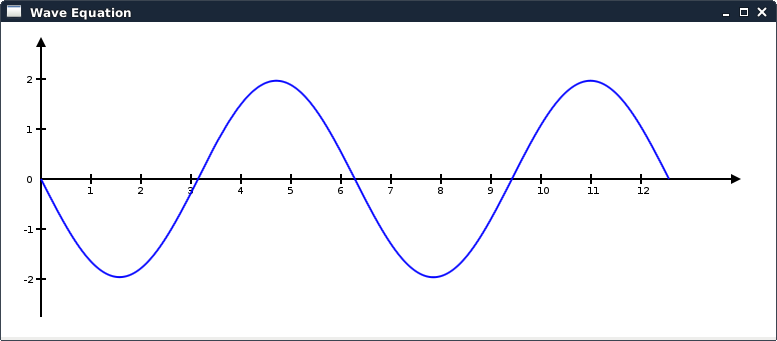
\includegraphics[width=0.9\textwidth]{pictures/gui}
	\caption{Graphical User Interface (GUI)}
	\label{fig:gui}
\end{figure}